\documentclass[11pt,a4paper]{article}
\usepackage[utf8]{inputenc}
\usepackage{amsmath,amssymb,amsthm}
\usepackage{tikz}
\usetikzlibrary{calc}
\usetikzlibrary{math}
\usetikzlibrary{shapes.geometric}
\usetikzlibrary{patterns}
\usetikzlibrary{arrows.meta}
\providecommand{\tikzpicture}{\comment}

\newcommand{\Vnew}{V_{\operatorname{new}}}

\begin{document}

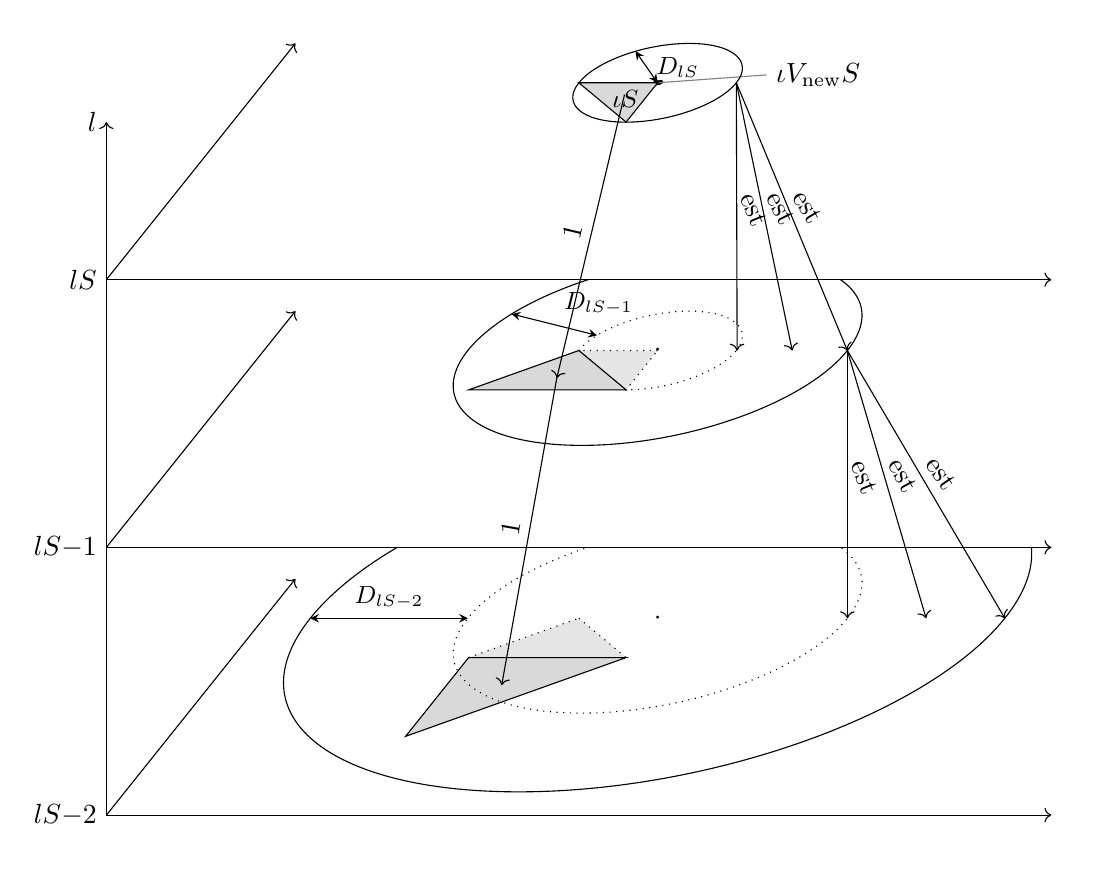
\begin{tikzpicture}[information text/.style={fill=gray!10,inner sep=1ex}, scale=2]
\def\a{.5};
\def\b{0};
\def\breite{12};
\def\c{.2};
\def\d{.25};
\def\e{0};
\def\y{1.7};
\def\n{2};
\def\factor{2};
\def\layer{
	\fill[white] (0,0) rectangle (12,8);
	\draw[->] (0,0) -- (\breite,0);
	\draw[->]  (0,0) -- (0,6);
};

\clip (-.5,-.2) rectangle (\a*\breite+.1,3.3+\y);
\draw[->] (0,0) node[left]{$lS{-}2$} -- (0,\n*\y+1) node[left]{$l$};

\begin{scope}[cm={\a,\b,\c,\d,(0,\e)}]
	\layer;
	\draw[fill=gray!20,dotted] (4,5) -- (5,4) --(3,4) -- cycle;
	\draw[fill=gray!30] (5,4) -- (3,4) --(3,2) -- cycle;
	\coordinate (c) at (8.41,5){};
	\coordinate (f) at (3.7,3.3){};
	\coordinate (g) at (1.5,1.5){};
	\coordinate (h) at (2.5,1.5){};
	\coordinate (i) at (2,1.75){};
	\coordinate (j) at (2,1.5){};
	\coordinate (k) at (2,2){};
	
	\draw (5,5) node {$\cdot$};
	\draw (5,5) circle [radius=4.41cm];
	\draw[dotted] (5,5) circle [radius=2.41cm];
	\draw[<->,>=stealth] (5-2.41*1,5+2.41*.0) -- node[above] {\small{$D_{lS{-}2}$}} (5-4.41*1,5+4.41*.0);
\end{scope}

\begin{scope}[yshift=\y cm]
\draw (0,0) node[left]{$lS{-}1$};
\begin{scope}[cm={\a,\b,\c,\d,(0,\e)}]
	\layer;
	\coordinate (b) at (7.41,5){};
	\coordinate (e) at (4,4.3){};
	\draw (5,5) node {$\cdot$};
	\draw (5,5) circle [radius=2.41cm];
	\draw[dotted] (5,5) circle [radius=1cm];
	\draw[<->,>=stealth] (5-1*12/13,5+1*5/13) -- node[above right] {\small{$D_{lS{-}1}$}} (5-2.41*12/13,5+2.41*5/13);
	\draw[fill=gray!20,dotted] (5,5) -- (4,5) --(5,4) -- cycle; 
	\draw[fill=gray!30] (4,5) -- (5,4) --(3,4) -- cycle;
\end{scope}

\begin{scope}[yshift=\y cm]
\draw (0,0) node[left]{$lS$};
\begin{scope}[cm={\a,\b,\c,\d,(0,\e)}]
	\fill[white] (0,0) rectangle (10,10);
	\layer;
	\coordinate (A) at (2,2){};
	\fill (5,5) circle [radius=.7mm];
	\draw[thin,gray,text=black] (5,5)--(6.3,5.2) node [right]{$\iota\Vnew S$};
	\draw (5,5) circle [radius=1cm];
	\draw[<->,>=stealth] (5,5) -- node[right] {\small{$D_{lS}$}} (5-1*.6,5+1*.8);
	\coordinate (a) at (6,5){};
	\coordinate (d) at (4.7,4.7){};
	\draw[fill=gray!30] (5,5) -- (4,5) --(5,4) -- cycle; 
	\filldraw (4.75,4.6) node {\small{$\iota S$}};
\end{scope}%%3D
\end{scope}%%erster y shift

%%obere pfeile
\begin{scope}[cm={\a,\b,\c,\d,(0,\e)}]
	\foreach \x in {7.41,6.71,...,6}
		\draw[->] (a) -- node [sloped, %near end,
		above] {est} (\x,5);
\end{scope}%%3D
\end{scope}%%zweiter y shift

%%untere pfeile
\begin{scope}[cm={\a,\b,\c,\d,(0,\e)}]
	\foreach \x in {9.41,8.41,...,7.41}
		\draw[->] (b) -- node [sloped, %near end,
		above] {est} (\x,5);
\end{scope}%%3D

%%1-pfeile
\draw[->] (d) -- node [sloped, above] {1} (e);
\draw[->] (e) -- node [sloped,above%, near start
] {1} (f);

%(2.5,1.25),(1.5,1.5),(2.5,1.5),
%%(2,1.75),


\end{tikzpicture}

\end{document}